\documentclass[twocolumn]{article} 
\usepackage{tikz}
\usepackage{circuitikz}
\usepackage{amsmath}
\usepackage{amssymb}
\usepackage{blindtext}
\usepackage{multicol}
\usepackage{graphicx}
\usepackage{url}
\usepackage[spanish, english]{babel}
\usepackage{ragged2e}
\usepackage{blindtext}
\usepackage[T1]{fontenc}
\usepackage{titlesec}
\usepackage{authblk}
\usepackage{float}
\usepackage{pgfplots}
\usepackage{float}
\usepackage{graphicx}
\usepackage{tikz}
\usetikzlibrary {3d}

\newcommand{\DCsymbol}{
    \begin{tikzpicture}[scale=0.2]
        \draw[thick] (0,0) -- (1,0);      % Línea superior continua
        \draw[thick] (0.2,-0.3) -- (0.5,-0.3); % Segmento inferior izquierdo
        \draw[thick] (0.7,-0.3) -- (1,-0.3);   % Segmento inferior derecho
    \end{tikzpicture}
}

\pgfplotsset{compat=1.18}
\title{\vspace{-85pt}\rule{\textwidth}{1pt}\vspace{0.25cm}\\ \begin{minipage}{0.2\textwidth}
    
\includegraphics[width=0.9\textwidth]{figura/logo.jpg}
\end{minipage}\hfill \begin{minipage}{0.8\textwidth}
    APRENDIENDO A USAR EL MULTÍMETRO EN DOS CIRCUITOS DE CORRIENTE CONTINUA Y ANALIZANDO PICOS DE VOLTAJE Y PERIODO EN CORRIENTE ALTERNA
\end{minipage}\vspace{0.25cm} \rule{\textwidth}{0.5pt}}
\author{\begin{minipage}{0.6\textwidth}Rengifo Cabrera José Franco,\\
Vaella Alarcon Titasho Anderson,\\
Valera Navez Bruno Daniel\end{minipage}\hfill \begin{minipage}{0.4\textwidth}
    jfrengifoca@unitru.edu.pe\\
   tavaellaal@unitru.edu.pe\\
    vdvalerana@unitru.edu.pe
\end{minipage}}
\affil{Universidad Nacional de Trujillo}
\date{\today \vspace{0.25cm} \rule{\textwidth}{0.5pt}}
\titleformat{\section}[wrap]
{\normalfont\bfseries}
{\thesection.}{0.1em}{}

\titlespacing{\section}{12pc}{1.5ex plus .1ex minus .2ex}{1pc}
\begin{document}
\maketitle

\begin{otherlanguage}{spanish}
\begin{abstract} \noindent

\end{abstract}
\end{otherlanguage}

\begin{abstract} \noindent

\end{abstract}
\newpage
\section{Introducción} \noindent

\noindent El estudio y la medición de parámetros eléctricos, como el voltaje y la corriente, son fundamentales para comprender y manipular dispositivos y sistemas eléctricos. Dos de los tipos de corriente más comunes en el uso cotidiano son la corriente continua (CC) y la corriente alterna (CA). La corriente continua fluye de manera unidireccional, y es común en dispositivos que funcionan con baterías, como celulares, linternas y laptops, ya que estas fuentes generan energía constante sin cambios en dirección o magnitud \cite{garcia2020}. Por otro lado, la corriente alterna cambia de dirección periódicamente y es la forma de electricidad que se distribuye en los hogares y negocios, alimentando dispositivos como electrodomésticos y equipos de calefacción y aire acondicionado \cite{martinez2020}.\noindent
\\

\noindent Para medir estos parámetros eléctricos, se utiliza el multímetro, un dispositivo de medición indispensable en electrónica y electricidad. El multímetro permite verificar tanto el voltaje como la corriente en diferentes circuitos, siendo útil tanto para aficionados como para profesionales. Es especialmente relevante entender las mediciones en corriente continua y alterna, ya que cada tipo de corriente tiene características particulares que requieren de configuraciones y técnicas de medición específicas \cite{lee2021}. En el caso de la corriente alterna, también es importante considerar conceptos como el periodo y el pico de voltaje, que describen el comportamiento oscilatorio de la corriente \cite{wilson2020}.

\section{Marco Teórico}

\subsection*{Uso del Multímetro en Corriente Continua (CC)}

El multímetro es un dispositivo capaz de medir voltaje (en voltios), corriente (en amperios) y resistencia (en ohmios), y en algunos casos, otras magnitudes como la capacitancia o la frecuencia \cite{brown2018}. En el contexto de la corriente continua, el multímetro permite evaluar el voltaje y la corriente en sistemas que requieren una fuente de alimentación estable. El voltaje en corriente continua permanece constante en un valor determinado y siempre fluye en una sola dirección desde el polo negativo al positivo \cite{garcia2020}.\noindent
\\

\noindent Para medir el voltaje en corriente continua, se coloca el multímetro en modo de medición de voltaje DC (representado comúnmente como "V\DCsymbol") y se conecta en paralelo al componente o sección del circuito donde se desea medir el potencial. En cambio, para medir la corriente en un circuito de corriente continua, el multímetro debe colocarse en serie con el circuito en el modo de medición de corriente DC. Estos procedimientos son críticos para evitar daños al multímetro y obtener mediciones precisas \cite{yang2022}.


\subsection*{Uso del Multímetro en Corriente Alterna (CA)}

La corriente alterna es aquella en la que el flujo de electricidad cambia de dirección de manera periódica. La tensión en corriente alterna se representa con una onda senoidal que sube y baja a través de un eje de tiempo, lo que genera un comportamiento cíclico \cite{martinez2020}. Para medir el voltaje en corriente alterna, se coloca el multímetro en el modo de voltaje AC (frecuentemente indicado como "V~") y se conecta en paralelo a la carga o al circuito. En general, el multímetro muestra el valor RMS (Root Mean Square o valor eficaz) de la señal de CA, que es el equivalente en corriente continua de esa señal alterna en términos de potencia \cite{allen2022}.\noindent
\\

\noindent Es menos común que los multímetros midan la corriente alterna directamente, especialmente en valores altos, ya que se requiere de un diseño de circuito específico que suele ser más peligroso y difícil de implementar en condiciones cotidianas. Para ello, se emplean multímetros con pinzas de corriente alterna (pinzas amperimétricas), que miden indirectamente el flujo de corriente alterna a través de la detección de campos magnéticos alrededor del conductor \cite{chang2021}.

\subsection*{Picos de Voltaje y Periodo en Corriente Alterna}

Un aspecto distintivo de la corriente alterna es su variabilidad periódica en voltaje, la cual se caracteriza por picos de voltaje y su periodo. El pico de voltaje se refiere al valor máximo de voltaje positivo o negativo que alcanza la onda alterna en su ciclo; este valor es fundamental al diseñar dispositivos electrónicos, ya que determina la tolerancia de los componentes eléctricos a los cambios en la señal \cite{rodriguez2021}. El periodo, por otro lado, es el tiempo que tarda la señal de CA en completar un ciclo completo, y su valor es inversamente proporcional a la frecuencia de la señal (medida en Hertz, Hz). La frecuencia estándar en la mayoría de los países es de 50 o 60 Hz, lo que significa que la corriente cambia de dirección 50 o 60 veces por segundo \cite{perez2019}.\noindent 
\\

\noindent Estos conceptos de pico de voltaje y periodo son esenciales en aplicaciones prácticas como en el diseño de fuentes de alimentación y en la transmisión de energía eléctrica a larga distancia. Comprender estos factores permite que los ingenieros y técnicos optimicen el diseño de circuitos para hacerlos más eficientes y seguros \cite{wilson2020}.

\section{Objetivos}
\begin{enumerate}
    \item Medir la intensidad de campo magnético al cambiar la corriente que lo induce.
    \item Encontrar la ecuación que describa la relación entre la intensidad de campo magnético que produce una corriente que pasa por una espira circular. 
\end{enumerate}

\section{Desarrollo experimental}
     \subsection{Instrumentos}
        \begin{itemize}
            \item Osciloscopio (Resolución de 0.001ms y 0.01V)
            \item Multímetro usado como amperímetro (resolución de 0.01 A).
            \item Multímetro usado como voltímetro (resolución de 0.01 v).
            \item Generador de funciones (Resolución de 1Hz y 0.001 Vpp)

        \end{itemize}
     \subsection{Materiales}

        \begin{itemize}
            \item Cables conectores
            \item Cable coaxial
            \item Modulo de estudio de circuitos en corriente continua
        \end{itemize}


\subsection{Metodología}
Usamos un modulo de estudio de circuitos en corriente continua para crear los circuitos que usaremos en
1 y 2.
\textbf{Experimento 1:}
Conectamos el circuito tal cual se ve en la figura del diseño experimental. Luego medimos corriente y voltaje en 

   \subsection*{Diseño experimental}

   \begin{figure}[htb]
    \centering
    \begin{circuitikz}[american voltages]
        \draw 
        (0,2) to [V, l=$\epsilon$] (0,-2)
        (0,2) -- (4,2)
        -- (4,1)
        -- (3,1)
        (3,1) to [R, l=$R_1$] (3,-1)
        -- (4,-1)
        (4,1) -- (5,1)
        to [R, l=$R_2$] (5,-1)
        -- (4,-1)
        -- (4,-2)
        -- (0,-2);
    \end{circuitikz}
\end{figure}


\section{Datos experimentales:} 

\begin{table}[H]
    \centering
    \begin{tabular}{|l|l|l|l|}
    \hline
    fuente/voltaje & $V_{\epsilon}$ (V) & $V_{R1}$ (V) & $V_{R2}$ (V) \\ \hline
    $\epsilon$_1 & 1.864 & 1.859 & 1.859 \\ \hline
    $\epsilon$_2 & 5.800 & 5.780 & 5.780 \\ \hline
    $\epsilon$_3 & 8.450 & 8.420 & 8.420 \\ \hline
    \end{tabular}
    \caption{Datos de voltaje en el primer circuito.}
\end{table}

\begin{table}[H]
    \centering
    \begin{tabular}{|l|l|l|l|}
    \hline
        I (A) & $I_{1}$ (A) & $I_{2}$ (A) \\ \hline
        7.50 & 1.87 & 5.56 \\ \hline
        23.60 & 5.86 & 17.36 \\ \hline
        34.50 & 8.50 & 26.00 \\ \hline
    \end{tabular}
    \caption{Datos de intensidad de corriente en el primer circuito}
\end{table}

\begin{table}[H]
    \centering
    \begin{tabular}{|l|l|}
    \hline
        $I_{1}$ (mA) & 3.5 \\ \hline
        $I_2$ (mA) & 0.61 \\ \hline
        $I_3$ (mA) & 2.6 \\ \hline
        $I_4$ (mA) & 3.5 \\ \hline
        $\epsilon$ (V) & 13.5 \\ \hline
        $\Delta$$V_1$ (V) & 3.4 \\ \hline
        $\Delta$$V_2$ (V) & 5.9 \\ \hline
        $\Delta$$V_3$ (V) & 5.9 \\ \hline
        $\Delta$$V_4$ (V) & 5.1 \\ \hline
    \end{tabular}
    \caption{tabla de datos del segundo circuito}
\end{table}

\section{Resultados:}

\section{Análisis y discusión}

\section{Conclusiones}
\begin{enumerate}
   \item 
\end{enumerate}


   
\begin{otherlanguage}{spanish}

\begin{thebibliography}{99}

\bibitem{allen2022} Allen, B. (2022). \textit{Electric Circuits and Measurements}. Boston: Prentice Hall.

\bibitem{brown2018} Brown, T. (2018). \textit{Principles of Electrical Engineering}. New York: McGraw-Hill.

\bibitem{chang2021} Chang, H. (2021). \textit{Electric Power and Machinery Fundamentals}. Singapore: World Scientific Publishing.

\bibitem{garcia2020} García, F. (2020). "Cómo usar el multímetro en corriente continua". \textit{Tecnología y Ciencia Aplicada}, 8(4), pp. 34-40.

\bibitem{lee2021} Lee, J., \& Kim, H. (2021). "Uso de multímetros en electrónica básica". \textit{Journal of Electrical Measurements}, 10(3), pp. 125-130.

\bibitem{martinez2020} Martínez, P. (2020). "Corriente continua y alterna: aplicaciones y diferencias en la vida diaria". \textit{Revista de Electrónica y Electricidad}, 32(1), pp. 50-56.

\bibitem{perez2019} Pérez, L., \& Rivera, G. (2019). "Conceptos básicos de corriente alterna y sus aplicaciones". \textit{Journal of Energy Technology}, 5(2), pp. 41-45.

\bibitem{rodriguez2021} Rodríguez, M. (2021). "Medición de voltaje alterno: Técnicas y aplicaciones". \textit{Journal of Applied Electricity}, 15(2), pp. 67-72.

\bibitem{smith2019} Smith, R. (2019). \textit{Fundamentals of Electrical Measurements}. London: Oxford University Press.

\bibitem{wilson2020} Wilson, K. (2020). "Características del voltaje alterno: Picos y frecuencias". \textit{Electrical Engineering Review}, 14(1), pp. 30-35.

\bibitem{yang2022} Yang, L., \& Zhou, X. (2022). \textit{Basic Electronics and Instrumentation}. Beijing: Science Press.

\end{thebibliography}
\end{otherlanguage}

\vspace{-0.5cm}
\section{Anexos} 
.
\begin{otherlanguage}{spanish}

\begin{figure}[H]
    \centering
    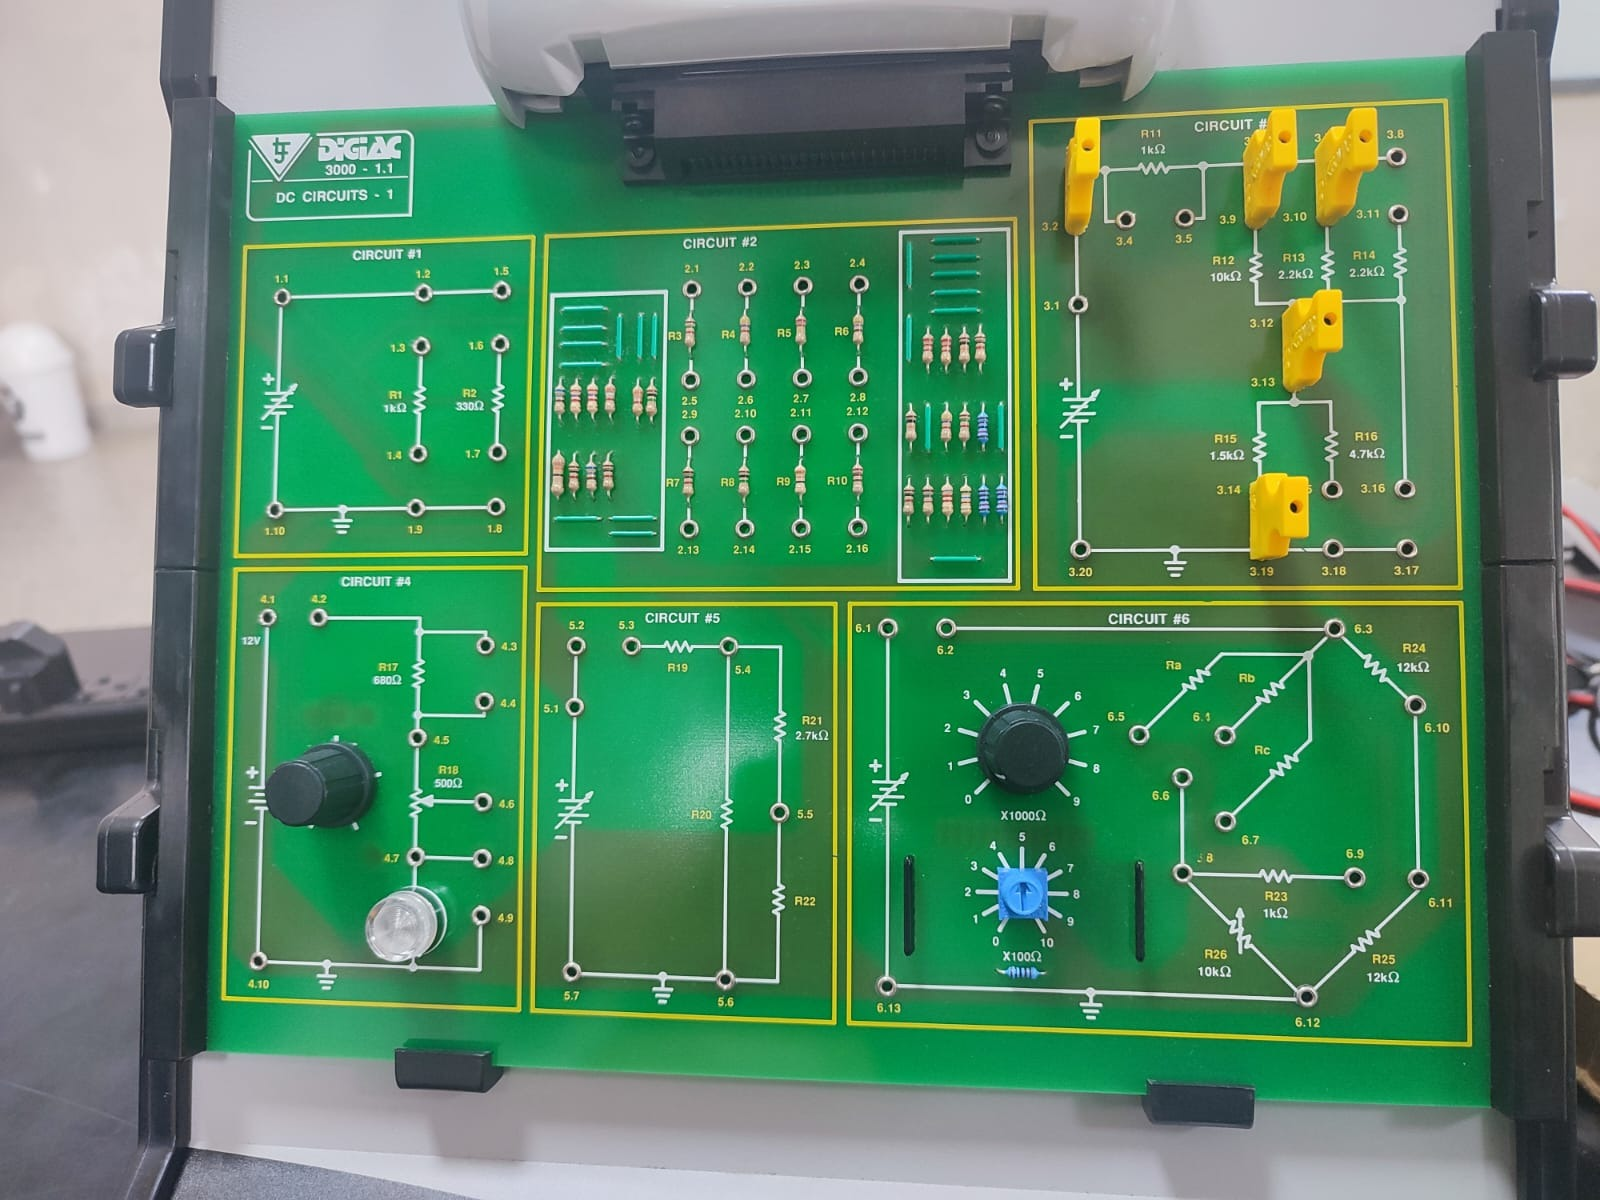
\includegraphics[width=0.7\linewidth]{Figures/figura/WhatsApp Image 2024-11-12 at 5.19.45 PM.jpeg}
    \caption{Modulo de estudio de circuitos en corriente continua}
    \label{}
\end{figure}

\begin{figure}[H]
    \centering
    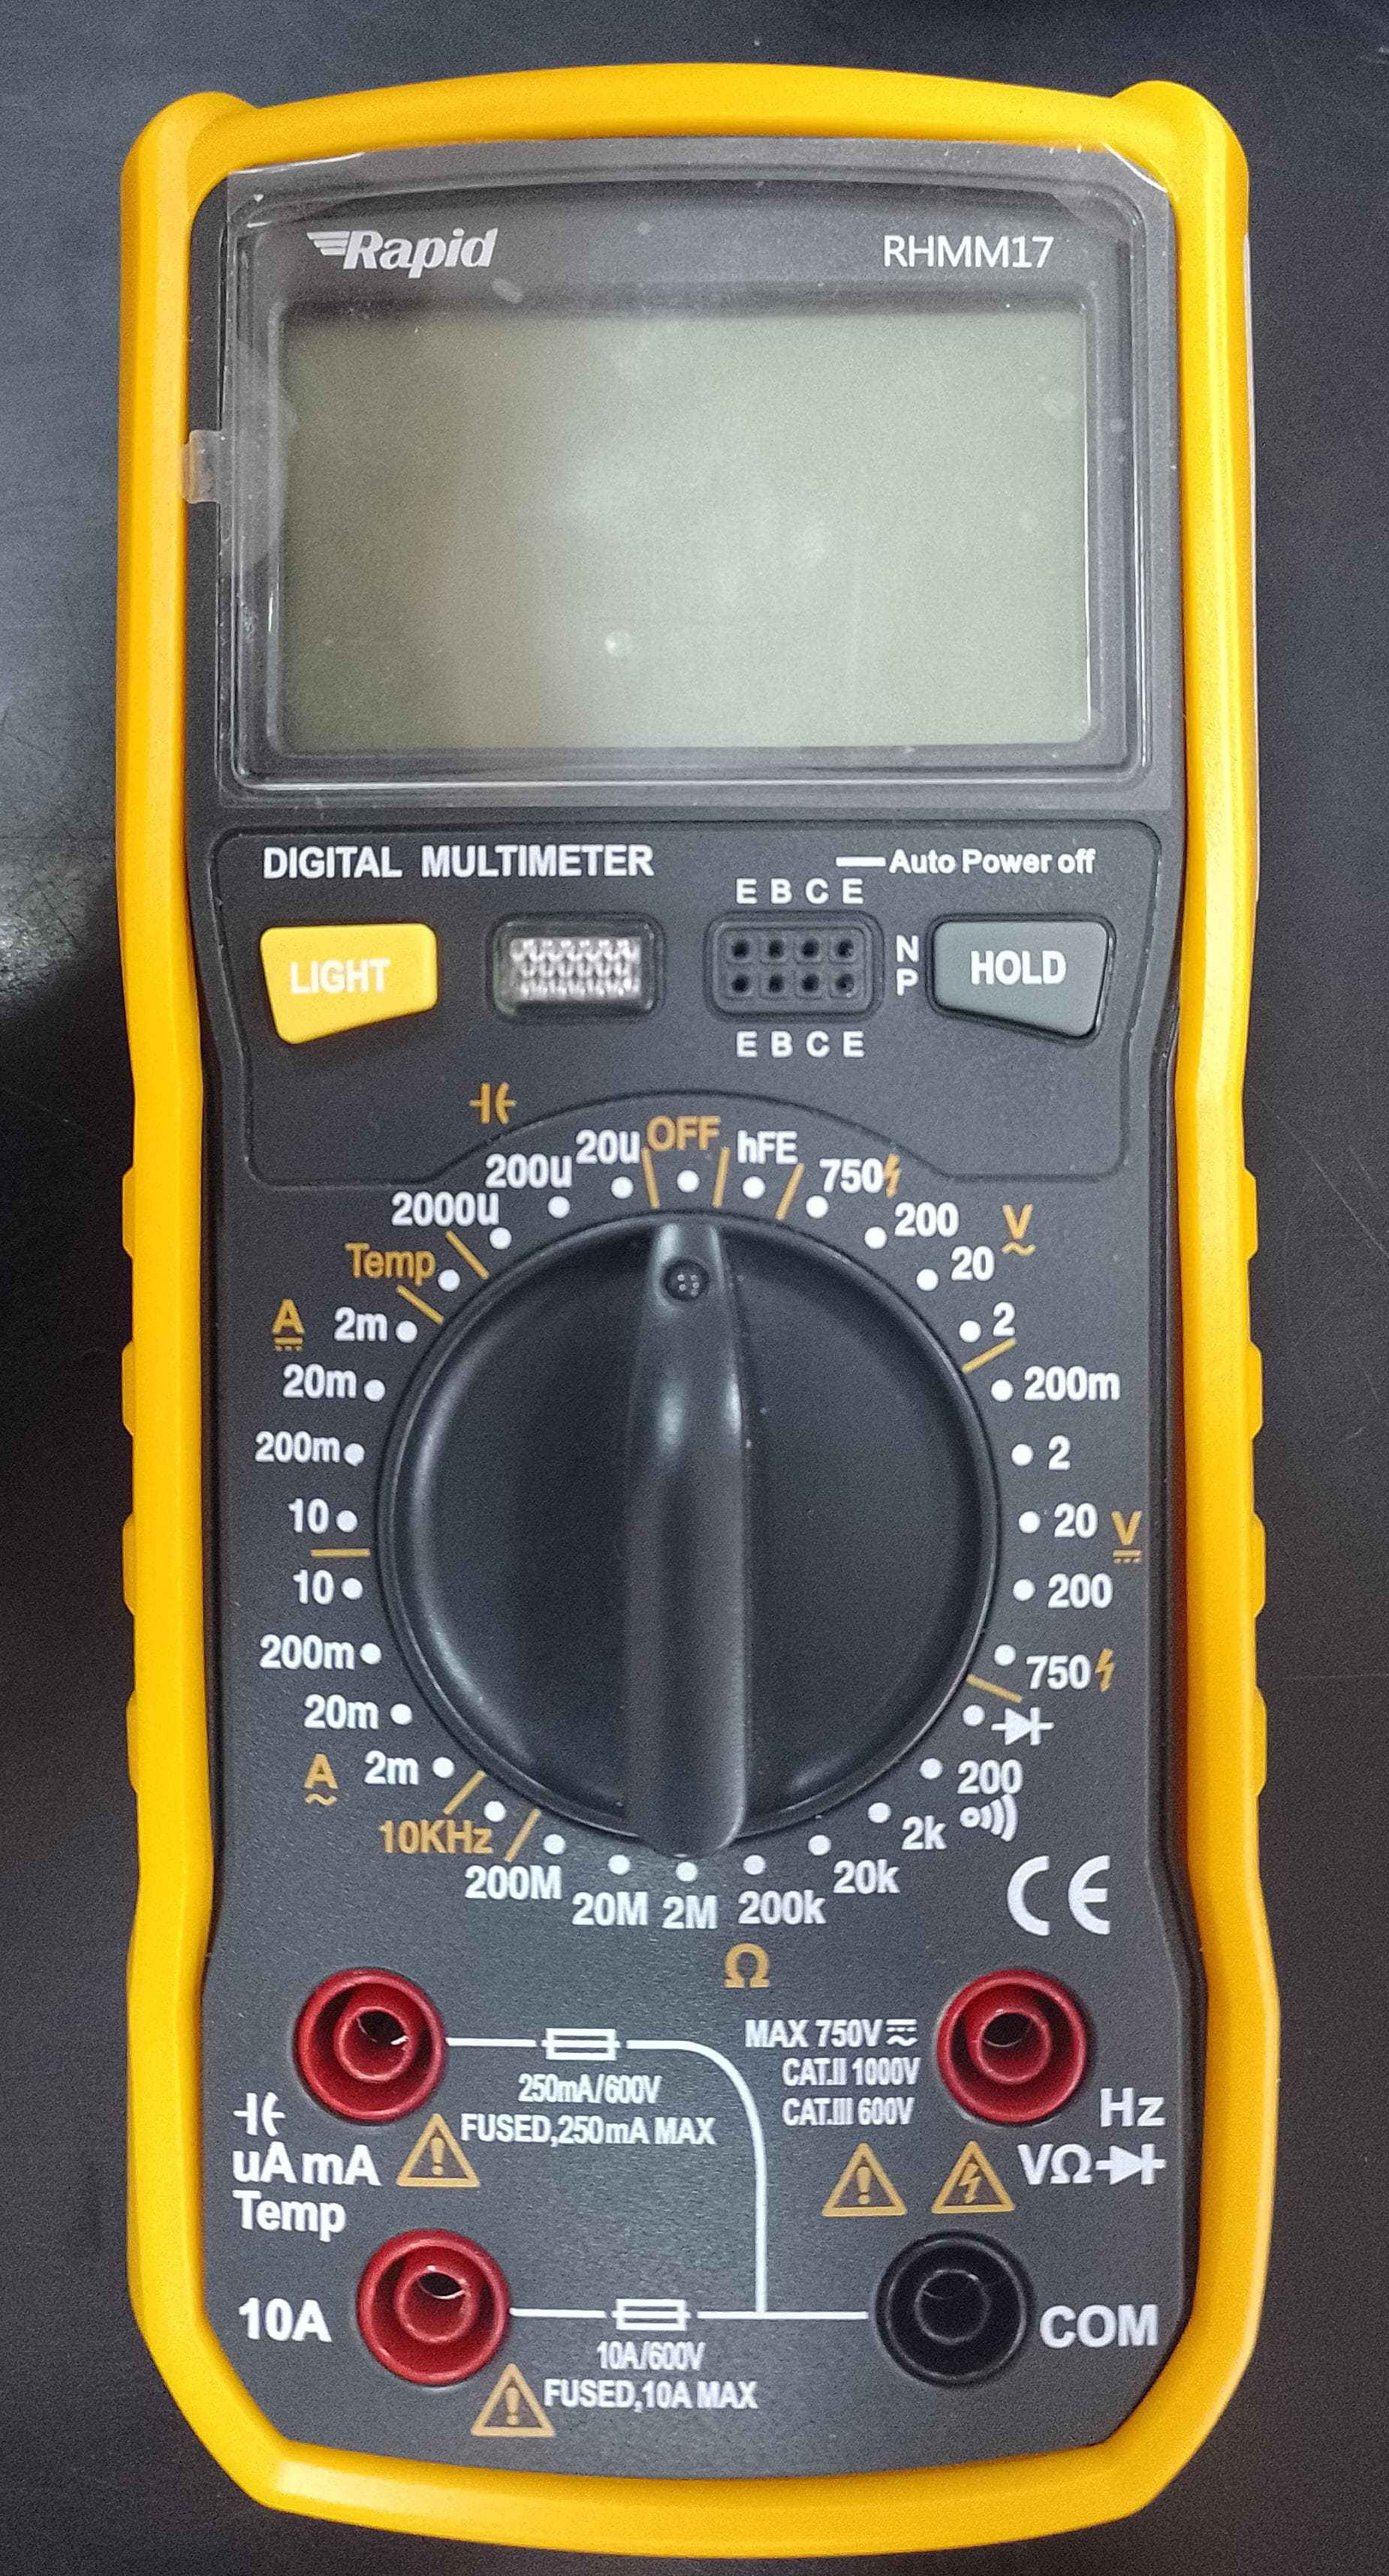
\includegraphics[width=0.3\linewidth]{Figures/figura/WhatsApp Image 2024-11-12 at 5.20.24 PM.jpeg}
    \caption{Multimetro}
    \label{}
\end{figure}

\begin{figure}[H]
    \centering
    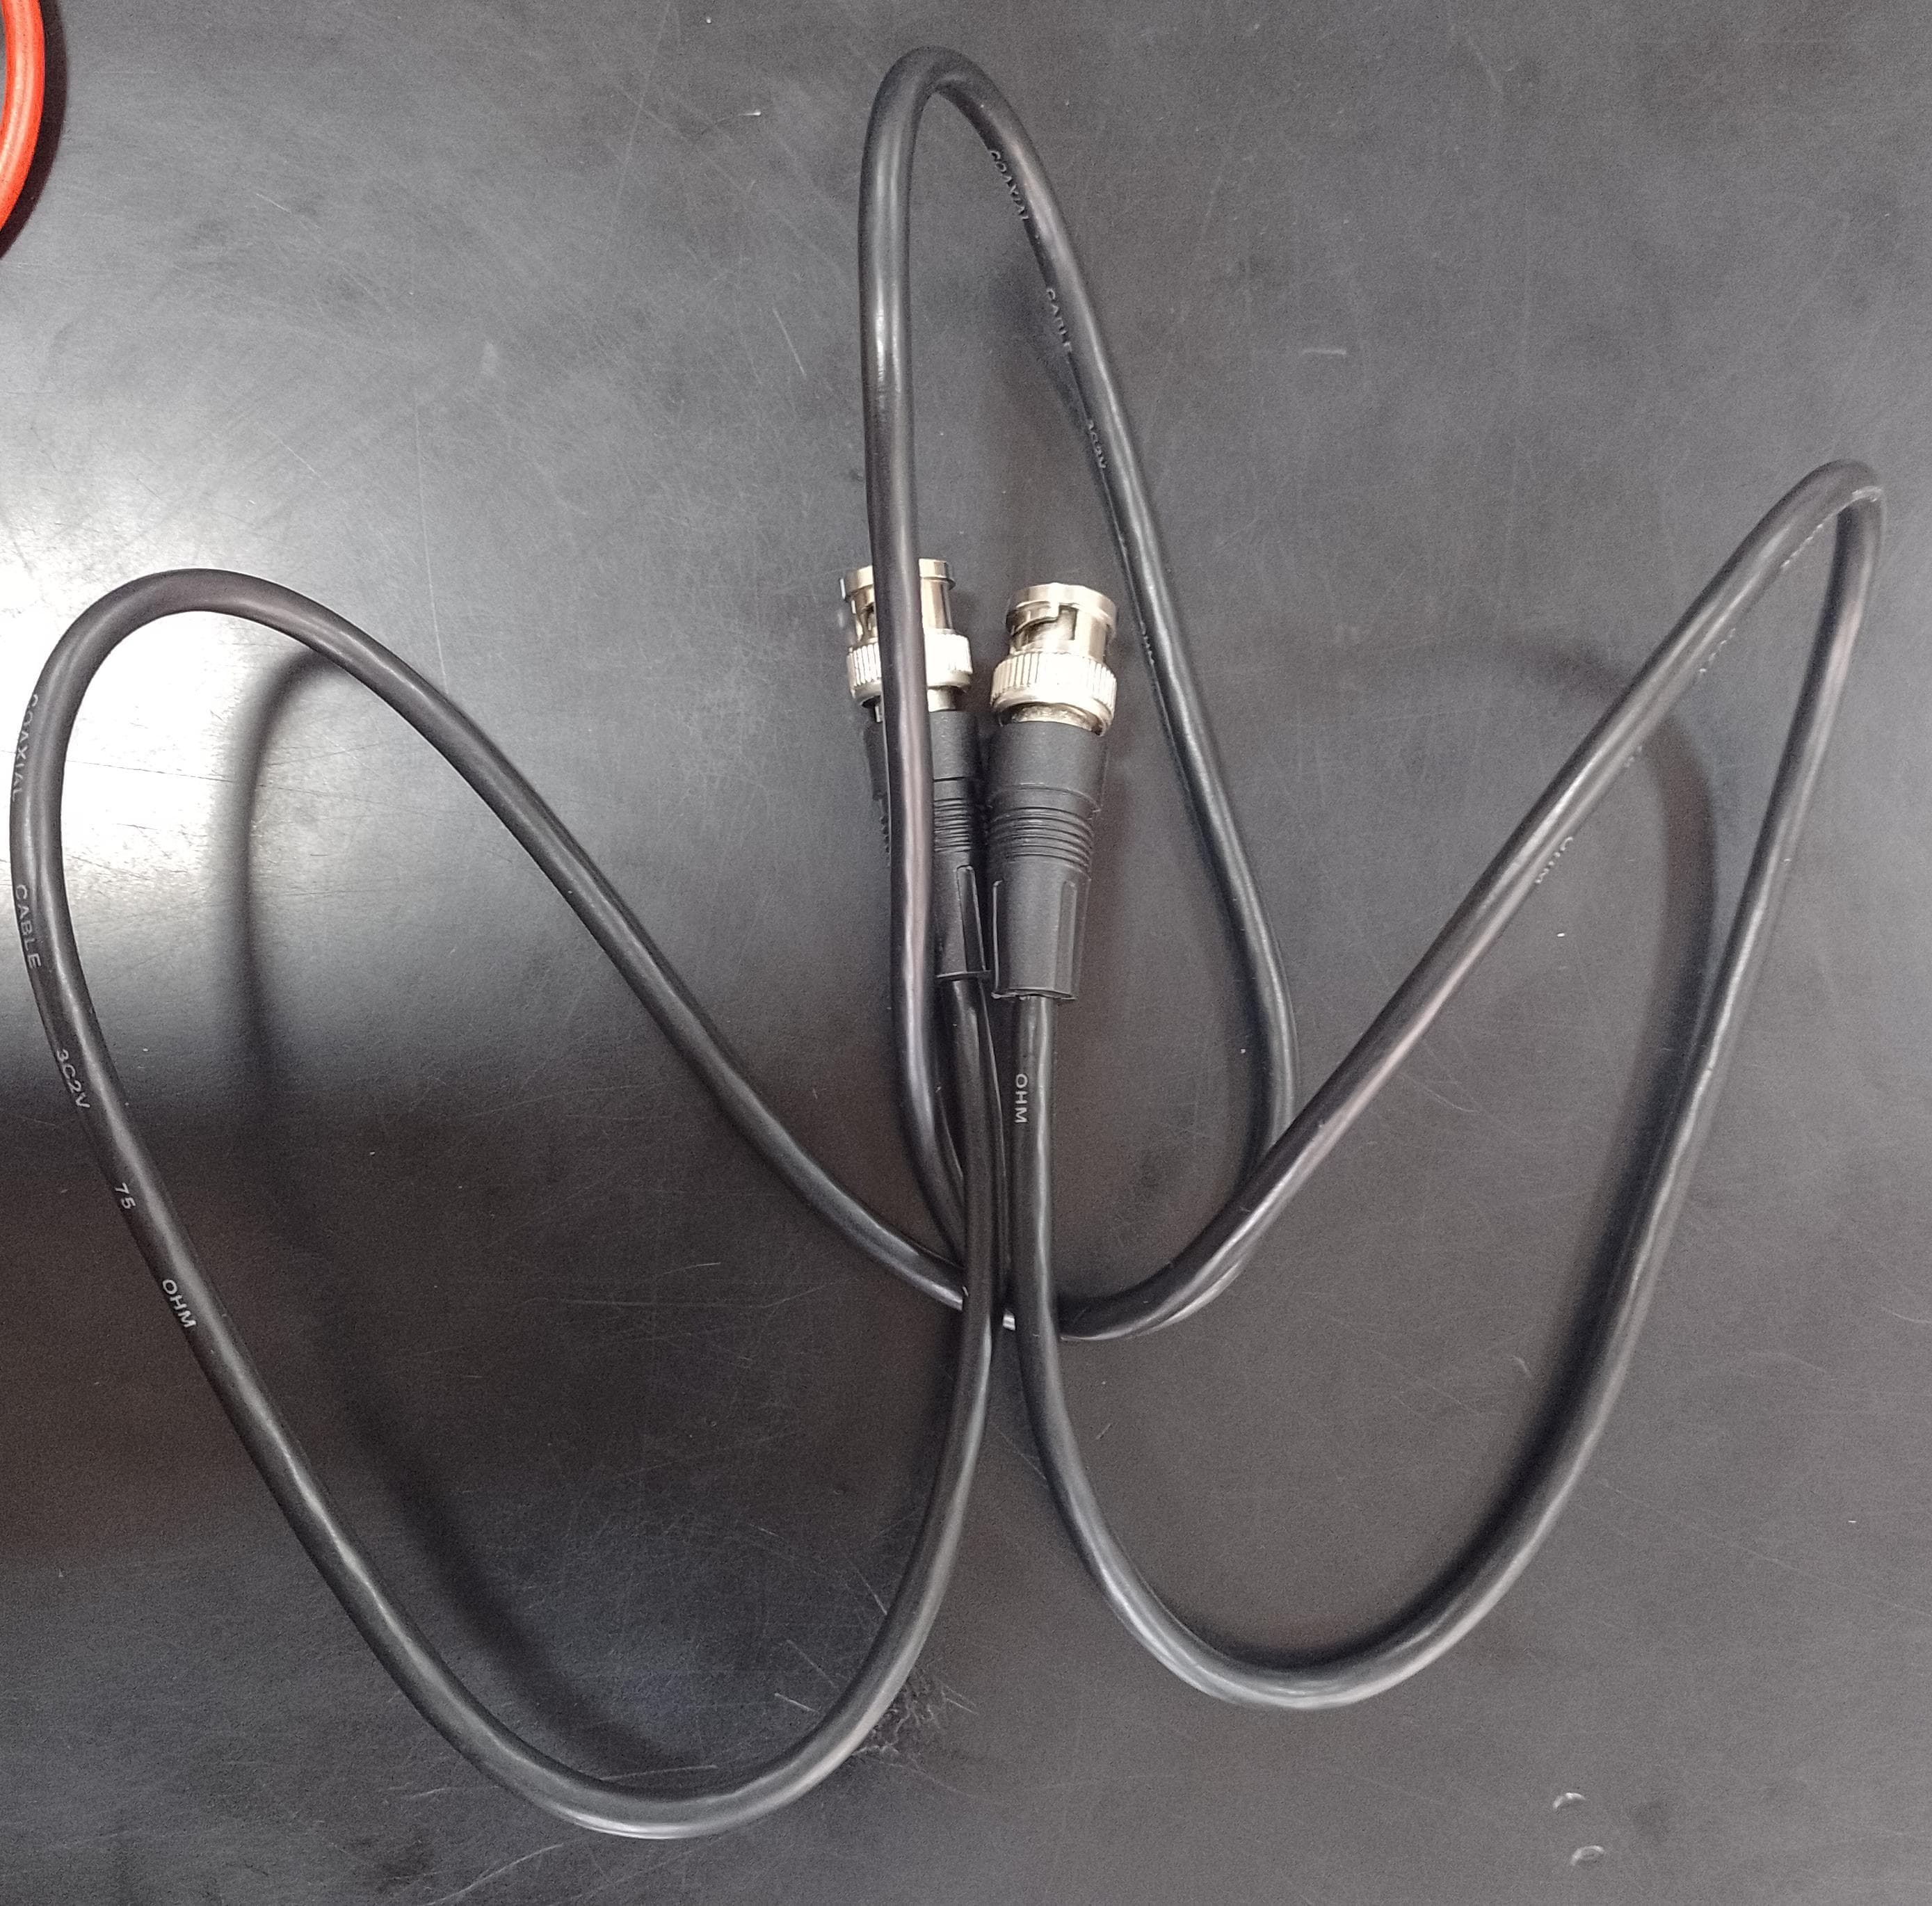
\includegraphics[width=0.6\linewidth]{Figures/figura/WhatsApp Image 2024-11-12 at 5.20.56 PM.jpeg}
    \caption{Cable coaxial}
    \label{}
\end{figure}

\begin{figure}[H]
    \centering
    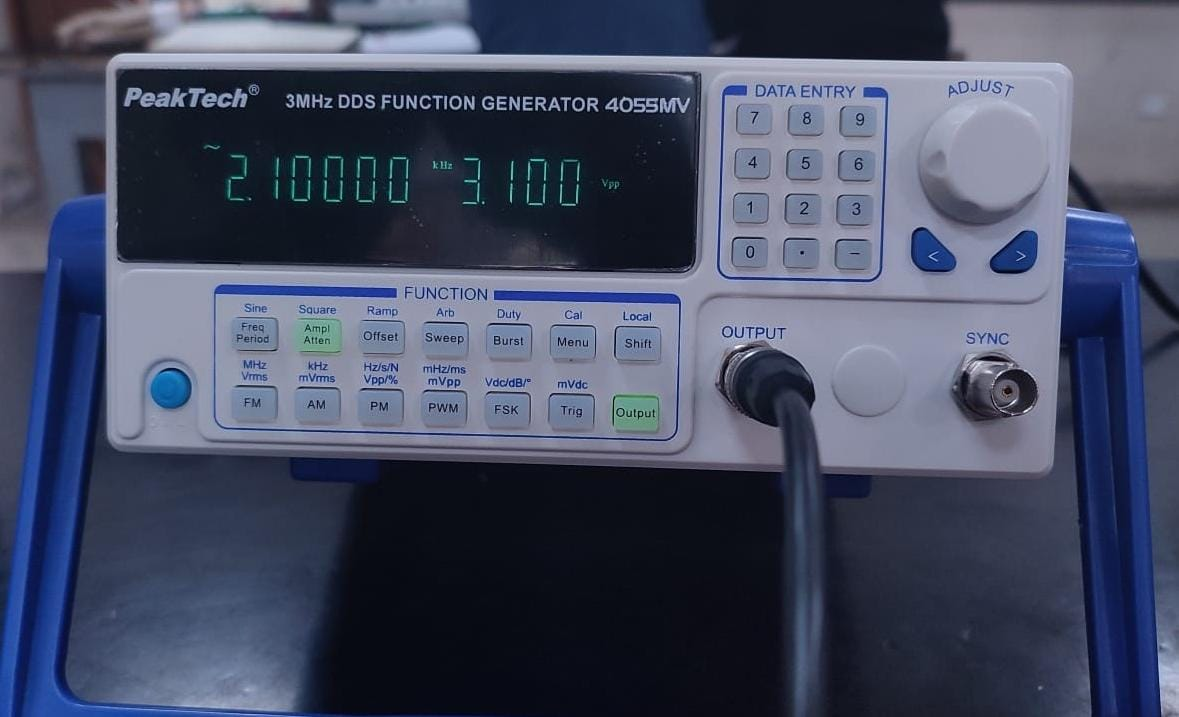
\includegraphics[width=0.8\linewidth]{Figures/figura/WhatsApp Image 2024-11-13 at 4.49.30 PM.jpeg}
    \caption{Generador de funciones}
    \label{}
\end{figure}

\begin{figure}[H]
    \centering
    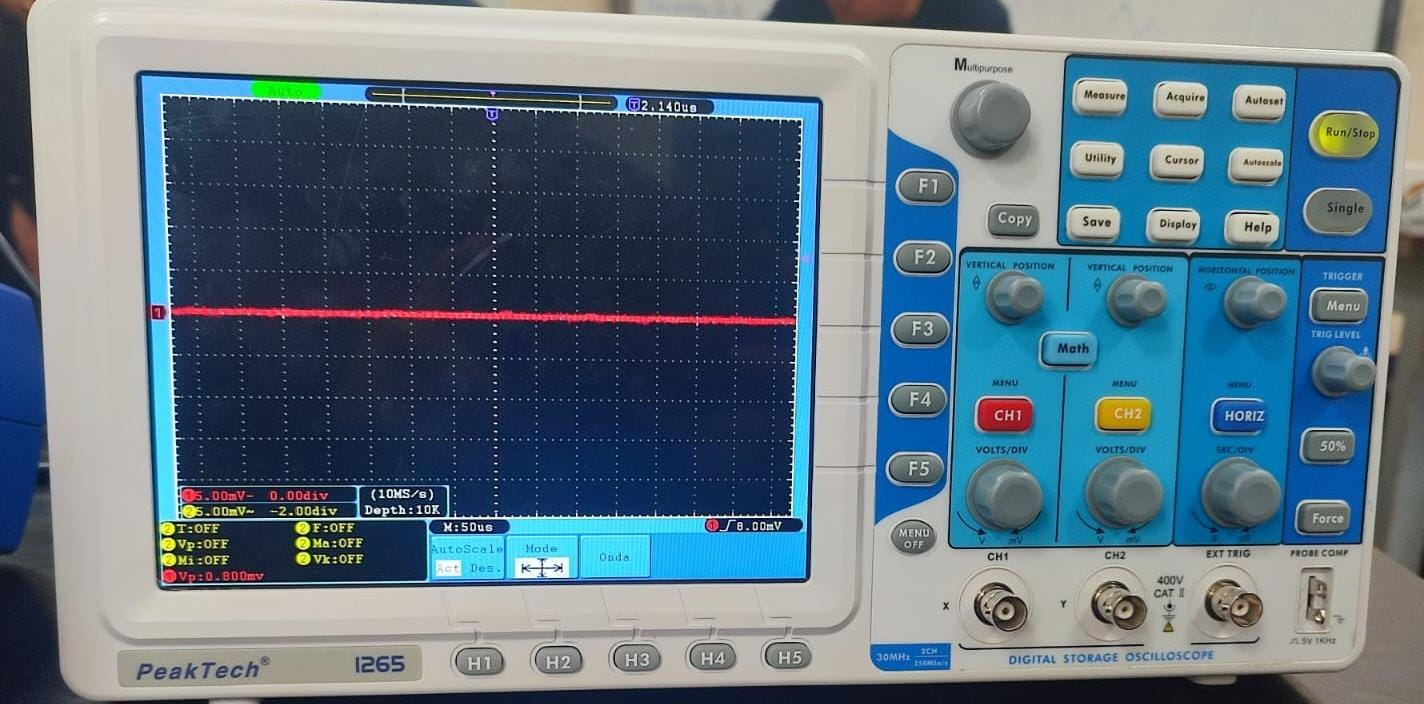
\includegraphics[width=0.9\linewidth]{Figures/figura/WhatsApp Image 2024-11-13 at 4.49.40 PM.jpeg}
    \caption{Osciloscopio}
    \label{}
\end{figure}

\begin{figure}[H]
    \centering
    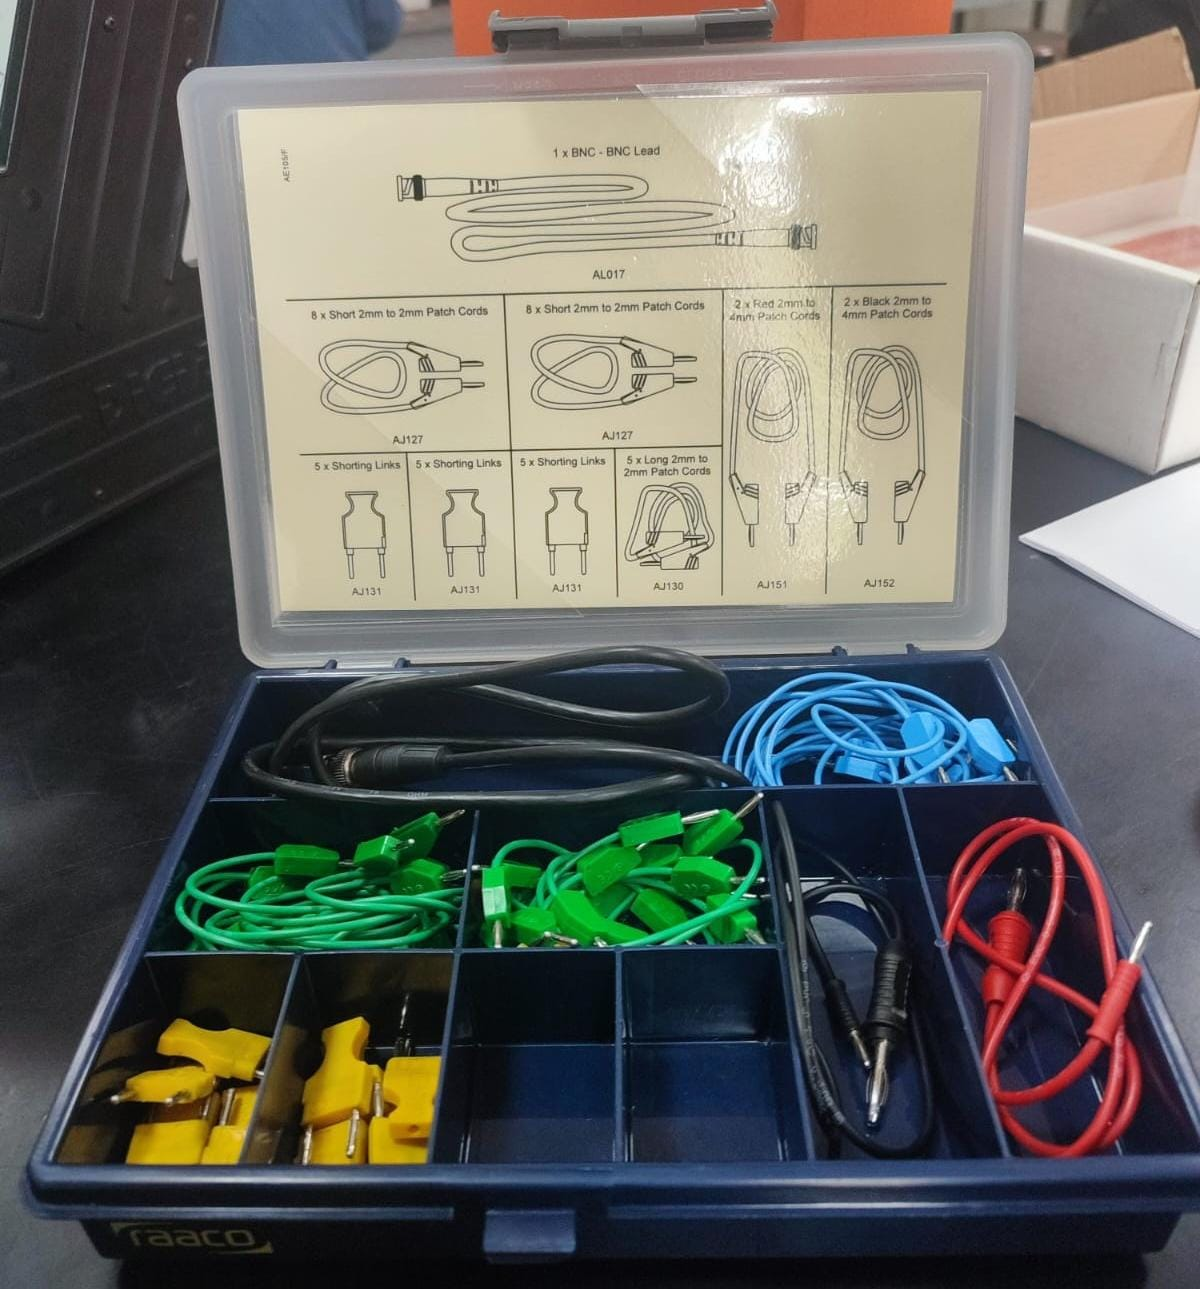
\includegraphics[width=0.8\linewidth]{Figures/figura/WhatsApp Image 2024-11-13 at 4.51.03 PM.jpeg}
    \caption{Cables conectores}
    \label{}
\end{figure}

\end{otherlanguage}

\end{document}
